%---PREMABLE BEGINS HERE------------------------

\documentclass[11pt]{article}
%------------------------
%------------------------
%Packages
\usepackage[top=0.75in, bottom=1.25in, left=1in, right=1in]{geometry} 
\usepackage{amsmath,amsthm,amssymb} %this is THE math package
\usepackage{mathtools} %an extension to the amsmath package that helps you write more beautiful math
\usepackage{enumitem} %for better control of your lists
\usepackage{hyperref} %for hyperlinking stuff
\usepackage{tikz}
\usetikzlibrary{hobby}
%------------------------
%Useful packages for more specialised use
%\usepackage{tikz}
%\usepackage{graphicx}
%\usepackage{fancybox}
%\usepackage{varwidth}
%\usepackage{mdframed}
%\usepackage{mathrsfs}
%------------------------
\usepackage{xcolor} %the ultimate package for defining various colours
\definecolor{firebrick}{RGB}{178,34,34}
\definecolor{teal}{RGB}{0,128,128}
\definecolor{indigo}{RGB}{75,0,130}
\definecolor{lightgrey}{RGB}{212, 212, 212}
\definecolor{darkblue}{rgb}{0.0,0.0,.7}
\definecolor{darkred}{rgb}{0.7,0.0,0.0}
\definecolor{darkgreen}{rgb}{0.0,0.3,0.0}
\definecolor{transparent}{HTML}{EDEFF0}
\definecolor{white}{HTML}{FAFAFA}
\definecolor{bluegrey}{HTML}{34495E}
%------------------------
%------------------------
%Fonts I use, uncomment if you like to use them.
%The first is the general font, and the second a math font
%the third one is more specialised
\usepackage{mathpazo}
%\usepackage{eulervm}
\usepackage[scr=boondox]{mathalfa}
%------------------------
%------------------------
%This is so that we have standard fonts for the doublestroked symbols
%for reals, naturals etc. regardless of what font you use.
%Don't comment
\AtBeginDocument{
  \DeclareSymbolFont{AMSb}{U}{msb}{m}{n}
  \DeclareSymbolFontAlphabet{\mathbb}{AMSb}}
%------------------------
%------------------------
%Environments
\newtheorem{theorem}{Theorem}[section]
\newtheorem{lemma}[theorem]{Lemma}

\theoremstyle{definition}
\newtheorem{definition}[theorem]{Definition}

\newtheorem{problem}{Problem}[section]
%------------------------
%------------------------
%User-defined notations
\newcommand{\zz}{\mathbf Z}   %bold Z
\newcommand{\qq}{\mathbf Q}   %bold Q
\newcommand{\ff}{\mathbf F}   %bold F
\newcommand{\RR}{\mathbb R}   %blackboard bold R
\newcommand{\rr}{\mathbf R}   %bold R
\newcommand{\nn}{\mathbf N}   %bold N
\newcommand{\cc}{\mathbf C}   %bold C
\newcommand{\af}{\mathbf A}   %bold A
\newcommand{\pp}{\mathbf P}   %bold P
\newcommand{\id}{\operatorname{id}} %for identity map
\newcommand{\im}{\operatorname{im}} %for image of a function
\newcommand{\dom}{\operatorname{dom}} %for domain of a function
\newcommand{\cat}[1]{\mathscr{#1}}   %calligraphic category
\newcommand{\abs}[1]{\left\lvert#1\right\rvert} %for absolute value
\newcommand{\norm}[1]{\left\lVert#1\right\rVert} %for norm
\newcommand{\modar}[1]{\operatorname{mod}{#1}} %for modular arithmetic
\newcommand{\set}[1]{\left\{#1\right\}} %for set
\newcommand{\setp}[2]{\left\{#1\ \middle|\ #2\right\}} %for set with a property
%------------------------
%------------------------
%Re-defined notations
\renewcommand{\epsilon}{\varepsilon}
\renewcommand{\displaystyle}{\disp}
%\renewcommand{\phi}{\varphi}
\renewcommand{\emptyset}{\varnothing}
\renewcommand{\geq}{\geqslant}
\renewcommand{\leq}{\leqslant}
\renewcommand{\Re}{\operatorname{Re}}
\renewcommand{\gcd}{\operatorname{GCD}}
\renewcommand{\Im}{\operatorname{Im}}
%\renewcommand{\qedsymbol}{$\blacksquare$}
%------------------------
%------------------------
\allowdisplaybreaks
\setlength\parindent{0pt} %controls indentation after paragraph break
%------------------------
%------------------------

%---PREAMBLE ENDS HERE------------------------


%---DOCUMENT BEGINS HERE------------------------
\begin{document}
 
\title{\texttt{tikz} Canvas}
\author{You}
\date{\today} 
\maketitle

%Use \[...\] instead of $$...$$

We add \verb!\usepackage{tikz}! to the Preamble. Consider the following figures. Investigate the code, tinker with it and see what pieces of the code does what.

\[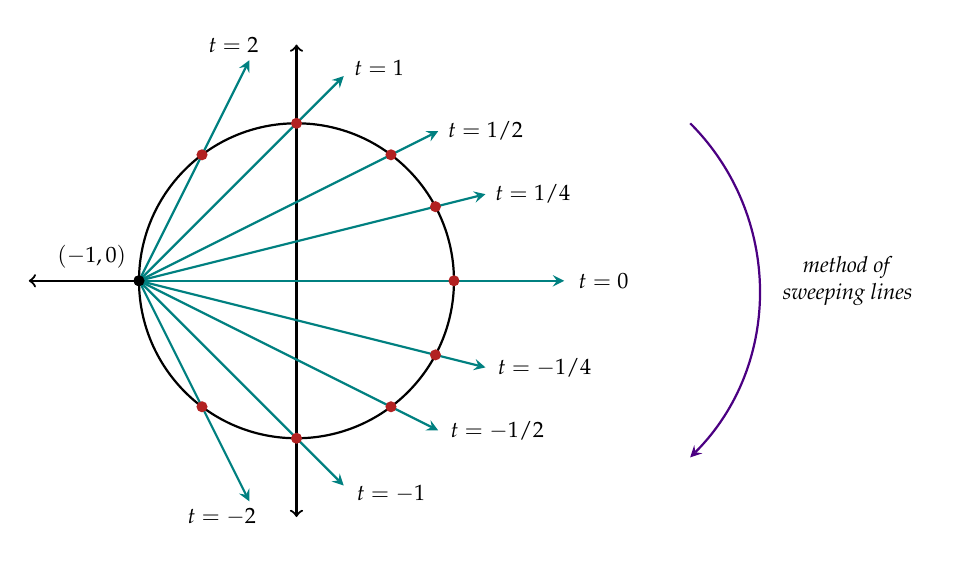
\begin{tikzpicture}[scale=2]
    \draw[<-,thick] (-1.7,0)--(-1,0);
    \draw[<->,thick] (0,-1.5)--(0,1.5);
    \draw[thick](0,0) circle (1);
    \fill (-1,0) circle (1pt);
	\draw[->,thick,>=stealth, color=teal] (-1,0)--(-0.3,1.4); %t = 2
    \fill[color=firebrick] (-0.6,0.8) circle (1pt); %t = 2
    \draw[->,thick,>=stealth, color=teal] (-1,0)--(0.3,1.3); %t = 1
    \fill[color=firebrick] (0,1) circle (1pt); %t = 1
    \draw[->,thick,>=stealth, color=teal] (-1,0)--(0.9,0.95); %t = 1/2
    \fill[color=firebrick] (0.6,0.8) circle (1pt); %t = 1/2
    \draw[->,thick,>=stealth, color=teal] (-1,0)--(1.2,0.55); %t = 1/4
    \fill[color=firebrick] (0.882352941,0.470588235) circle (1pt); %t = 1/4
    \draw[->,thick,>=stealth, color=teal] (-1,0)--(1.7,0); %t = 0
    \fill[color=firebrick] (1,0) circle (1pt); %t = 0
	\draw[->,thick,>=stealth, color=teal] (-1,0)--(-0.3,-1.4); %t = -2
    \fill[color=firebrick] (-0.6,-0.8) circle (1pt); %t = -2
    \draw[->,thick,>=stealth, color=teal] (-1,0)--(0.3,-1.3); %t = -1
    \fill[color=firebrick] (0,-1) circle (1pt); %t = -1
    \draw[->,thick,>=stealth, color=teal] (-1,0)--(0.9,-0.95); %t = -1/2
    \fill[color=firebrick] (0.6,-0.8) circle (1pt); %t = -1/2
    \draw[->,thick,>=stealth, color=teal] (-1,0)--(1.2,-0.55); %t = -1/4
    \fill[color=firebrick] (0.882352941,-0.470588235) circle (1pt); %t = -1/4
    \fill (-1,0) circle (1pt);
	\node[] at (-1.3,0.15) {\footnotesize$(-1,0)$};
    \node[] at (-0.4,1.5) {\footnotesize $t=2$};
    \node[] at (-0.475,-1.5) {\footnotesize $t=-2$};
    \node[] at (0.525,1.35) {\footnotesize $t=1$};
    \node[] at (0.6,-1.35) {\footnotesize $t=-1$};
    \node[] at (1.2,0.95) {\footnotesize $t=1/2$};
    \node[] at (1.275,-0.95) {\footnotesize $t=-1/2$};
    \node[] at (1.5,0.55) {\footnotesize $t=1/4$};
    \node[] at (1.575,-0.55) {\footnotesize $t=-1/4$};
    \node[] at (1.95,0) {\footnotesize $t=0$};
	\draw[->,>=stealth,thick,color=indigo] (1.5,1) (2.5,1) arc(225:135:-1.5);
    \node[] at (3.5,0) {\footnotesize\begin{tabular}{c}\emph{method of}\\ \emph{sweeping lines}\end{tabular}};
\end{tikzpicture}\]
\\
\[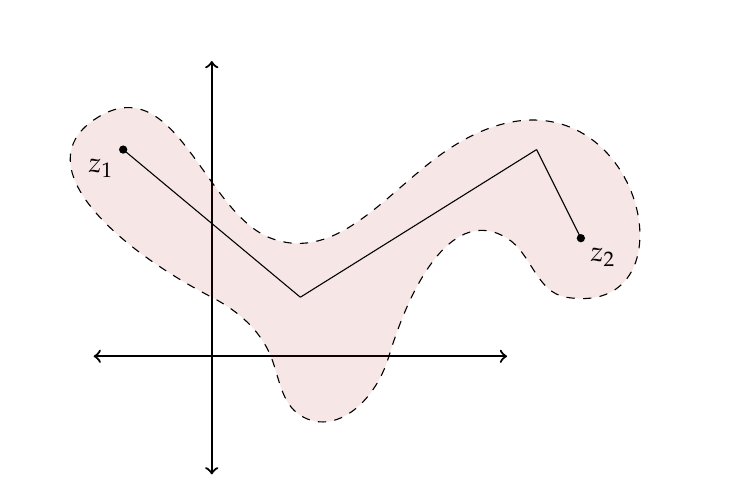
\begin{tikzpicture}[scale=0.75]
    \draw[<->,thick] (-2,0)--(5,0);
	\draw[<->,thick] (0,-2)--(0,5);
    \path[draw,use Hobby shortcut,closed=true,fill=darkred,fill opacity=1/10,dashed]
(-2,4) .. (1,2) .. (4,3.5) .. (6,1) .. (5,2) .. (3,0) .. (1.5,-1) .. (1,0) .. (0,1) .. (-2,4);
    \draw[](-1.5,3.5)--(1.5,1);
    \draw[](1.5,1)--(5.5,3.5);
    \draw[](5.5,3.5)--(6.25,2);
    \fill (-1.5,3.5) circle (2pt) node[below left]{$z_1$};
    \fill (6.25,2) circle (2pt) node[below right]{$z_2$};
\end{tikzpicture}\]
\\
For more information, google specific keywords, head to the whatever \href{https://tex.stackexchange.com/}{\color{darkblue}\TeX\ Stackexchange} article shows up. Copy the code and experiment!\\
\\
For this session, to begin with, try drawing the figure on the blackboard.

%---DOCUMENT ENDS HERE------------------------
\end{document}
